\documentclass[12pt]{article}

% Packages
\usepackage[margin=2.5cm]{geometry}
\usepackage{amsmath}
\usepackage{amssymb}
\usepackage{bm}
\usepackage{graphicx}
\usepackage{physics}
\usepackage{tikz}
\usetikzlibrary{arrows.meta, positioning, shapes.geometric}

% Better boxes
\usepackage{amsfonts}

% No indentation
\setlength{\parindent}{0pt}
\setlength{\parskip}{6pt}

\begin{document}

	\title{Guidelines for Adsorption Isotherm Models}
	\maketitle

	\tableofcontents
	\newpage

	\section{Langmuir isotherm}
	
	The Langmuir isotherm is usually written as
	\begin{equation}
		q_e = \frac{Q_{\max} K_L C_e}{1 + K_L C_e},
		\label{eq:Langmuir}
	\end{equation}
	where \(q_e\) is the equilibrium adsorbed amount, \(C_e\) is the equilibrium
	concentration in the fluid phase, \(Q_{\max}\) is the maximum adsorption
	capacity, and \(K_L\) is the Langmuir equilibrium constant.
	
	\subsection{High concentration limit, $Q_{max}$: \(C_e \to \infty\)}
	
	From eq.~\eqref{eq:Langmuir},
	\begin{equation}
		\lim_{C_e \to \infty} q_e
		= \lim_{C_e \to \infty}
		\frac{Q_{\max} K_L C_e}{1 + K_L C_e}.
	\end{equation}
	Dividing numerator and denominator by \(K_L C_e\) gives
	\begin{equation}
		\lim_{C_e \to \infty} q_e
		= Q_{\max} \lim_{C_e \to \infty}
		\frac{1}{\frac{1}{K_L C_e} + 1}
		%= Q_{\max} \cdot \frac{1}{0 + 1}
		= Q_{\max}.
	\end{equation}
	Therefore, the Langmuir isotherm saturates at
	\begin{equation}
		\boxed{\displaystyle \lim_{C_e \to \infty} q_e = Q_{\max}}.
	\end{equation}
	
	\subsection{Low concentration limit: Henry constant as the initial slope}
	
	For small \(C_e\), such that \(K_L C_e \ll 1\), the denominator of
	eq.~\eqref{eq:Langmuir} can be expanded:
	\begin{equation}
		\frac{1}{1 + K_L C_e} \approx 1 - K_L C_e + \mathcal{O}(C_e^2).
	\end{equation}
	Substituting into eq.~\eqref{eq:Langmuir} and keeping only the first order
	term in \(C_e\),
	\begin{equation}
		q_e \approx Q_{\max} K_L C_e.
	\end{equation}
	The Henry law form is
	\begin{equation}
		q_e \approx K_H C_e,
	\end{equation}
	so that the Henry constant is identified as the initial slope at
	\(C_e \to 0\):
	\begin{equation}
		K_H = \left.\frac{\mathrm{d}q_e}{\mathrm{d}C_e}\right|_{C_e \to 0}
		= Q_{\max} K_L.
	\end{equation}
	Thus,
	\begin{equation}
		\boxed{K_H = Q_{\max} K_L.}
	\end{equation}
	
	\subsection{Adsorption free energy}
	
	The Langmuir constant \(K_L\) is an equilibrium constant that can be
	related to the standard Gibbs free energy of adsorption. To make the
	constant dimensionless, one introduces a standard concentration
	\(C^0\) (typically \(1~\mathrm{mol~L^{-1}}\)) and defines
	\begin{equation}
		K_L^{\ast} = K_L C^0.
	\end{equation}
	The standard Gibbs free energy of adsorption is then
	\begin{equation}
		\Delta G_{\mathrm{ads}}^{0}
		= - R T \ln K_L^{\ast}
		= - R T \ln\left( K_L C^0 \right),
	\end{equation}
	where \(R\) is the gas constant and \(T\) is the absolute temperature.
	
	An adsorption affinity energy \(E_{\mathrm{aff}}\) can be naturally defined
	as the magnitude of this free energy:
	\begin{equation}
		E_{\mathrm{aff}} = - \Delta G_{\mathrm{ads}}^{0}
		= R T \ln\left( K_L C^0 \right).
	\end{equation}
	Therefore, the Langmuir constant provides a direct connection between
	the macroscopic isotherm parameters and the microscopic thermodynamic
	driving force for adsorption:
	\begin{equation}
		\boxed{\Delta G_{\mathrm{ads}}^{0}
			= - R T \ln\left( K_L C^0 \right),
			\qquad
			E_{\mathrm{aff}} = R T \ln\left( K_L C^0 \right).}
	\end{equation}
	
	\subsection{Energy distribution as a function of temperature}
	
	For a single Langmuir site, the adsorption affinity energy is
	\begin{equation}
		E_{\mathrm{aff}}(T)
		= R T \ln\!\left(K_L C^0\right),
		\label{eq:Eaff_def}
	\end{equation}
	where \(K_L\) is the Langmuir equilibrium constant, \(C^0\) is a standard
	concentration, \(R\) is the gas constant, and \(T\) is the absolute
	temperature.
	
	In a heterogeneous adsorbent, one can consider a continuous distribution of
	Langmuir constants \(K_L\), characterized by a normalized distribution
	function \(g(K_L)\),
	\begin{equation}
		\int_{0}^{\infty} g(K_L)\, \mathrm{d}K_L = 1.
	\end{equation}
	Using eq.~\eqref{eq:Eaff_def}, the energy and the equilibrium constant are
	related by
	\begin{equation}
		E = R T \ln\!\left(K_L C^0\right),
		\qquad
		K_L = \frac{1}{C^0} \exp\!\left(\frac{E}{R T}\right).
		\label{eq:K_of_E}
	\end{equation}
	
	The corresponding distribution of adsorption energies, \(f(E;T)\), is
	obtained by a change of variables,
	\begin{equation}
		f(E;T)\, \mathrm{d}E = g(K_L)\, \mathrm{d}K_L.
	\end{equation}
	Using eq.~\eqref{eq:K_of_E}, one has
	\begin{equation}
		\frac{\mathrm{d}K_L}{\mathrm{d}E}
		= \frac{1}{C^0} \frac{1}{R T}
		\exp\!\left(\frac{E}{R T}\right)
		= \frac{K_L(E,T)}{R T},
	\end{equation}
	so that
	\begin{equation}
		f(E;T)
		= g\!\left(K_L(E,T)\right)
		\frac{\mathrm{d}K_L}{\mathrm{d}E}
		= g\!\left(\frac{1}{C^0} \exp\!\frac{E}{R T}\right)
		\frac{1}{R T C^0}
		\exp\!\left(\frac{E}{R T}\right).
		\label{eq:f_E_T_general}
	\end{equation}
	
	Equation~\eqref{eq:f_E_T_general} shows explicitly how the energy
	distribution \(f(E;T)\) depends on temperature through both the exponential
	factor and the mapping \(K_L(E,T)\). If the intrinsic heterogeneity of the
	surface is represented by a temperature-independent distribution \(g(K_L)\),
	the apparent energy distribution observed in adsorption experiments still
	changes with \(T\) because higher-energy sites are progressively weighted by
	the Boltzmann-type factor \(\exp(E / R T)\).
	
	
	\begin{figure}
		\centering
		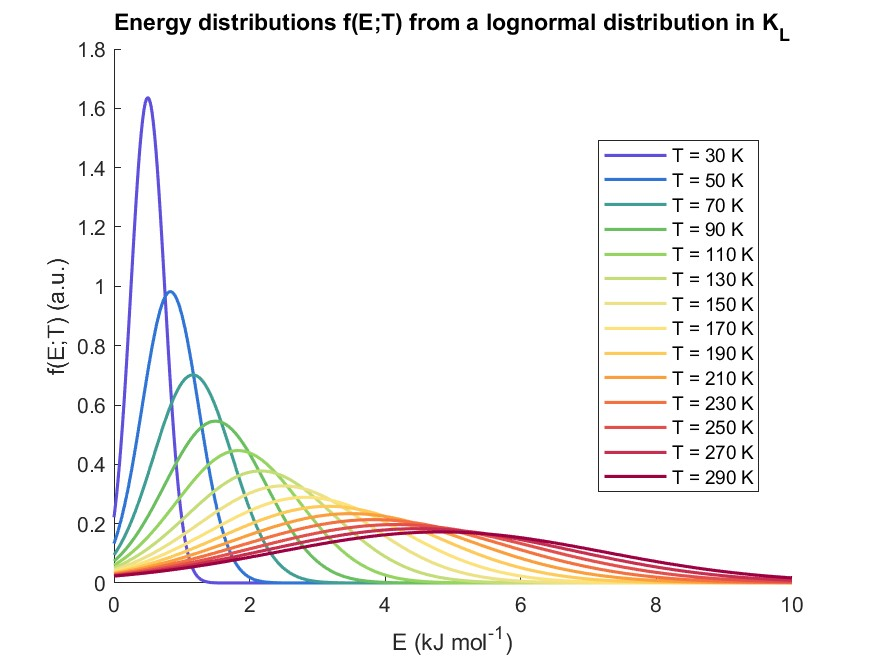
\includegraphics[width=0.75\linewidth]{Langmuir_energy.jpg}
		\caption{Energy distribution in function of energy for Langmuir isotherm}
		\label{fig:Langmuir_energy}
	\end{figure}
	
	\section{Double Langmuir}
	
	% Dual-site (Double) Langmuir isotherm: limits and Henry-law behavior
	
	The dual-site (double) Langmuir isotherm can be written as
	\begin{equation}
		q_e
		= \frac{Q_{\max,1} K_1 C_e}{1 + K_1 C_e}
		+ \frac{Q_{\max,2} K_2 C_e}{1 + K_2 C_e},
		\label{eq:DoubleLangmuir}
	\end{equation}
	where \(q_e\) is the equilibrium adsorbed amount, \(C_e\) is the
	equilibrium concentration in the fluid phase, \(Q_{\max,i}\) is the
	maximum adsorption capacity of site \(i\), and \(K_i\) is the Langmuir
	equilibrium constant for site \(i\) (with \(i = 1,2\)).
	
	\subsection{High concentration limit: \(C_e \to \infty\)}
	
	Consider the limit \(C_e \to \infty\) in eq.~\eqref{eq:DoubleLangmuir}.
	For each site,
	\begin{equation}
		\lim_{C_e \to \infty} \frac{Q_{\max,i} K_i C_e}{1 + K_i C_e}
		= Q_{\max,i} \lim_{C_e \to \infty}
		\frac{K_i C_e}{1 + K_i C_e}.
	\end{equation}
	Dividing numerator and denominator by \(K_i C_e\) gives
	\begin{equation}
		\lim_{C_e \to \infty} \frac{Q_{\max,i} K_i C_e}{1 + K_i C_e}
		= Q_{\max,i} \lim_{C_e \to \infty}
		\frac{1}{\frac{1}{K_i C_e} + 1}
		= Q_{\max,i} \cdot \frac{1}{0 + 1}
		= Q_{\max,i}.
	\end{equation}
	Therefore, the total loading at saturation is
	\begin{equation}
		\lim_{C_e \to \infty} q_e
		= Q_{\max,1} + Q_{\max,2}.
	\end{equation}
	Defining the total maximum capacity
	\begin{equation}
		Q_{\max}^{\mathrm{(tot)}} = Q_{\max,1} + Q_{\max,2},
	\end{equation}
	we obtain
	\begin{equation}
		\boxed{\displaystyle \lim_{C_e \to \infty} q_e
			= Q_{\max}^{\mathrm{(tot)}}.}
	\end{equation}
	
	\subsection{Low concentration limit: global Henry constant at \(C_e \to 0\)}
	
	For small \(C_e\), such that \(K_i C_e \ll 1\) for both sites,
	we can expand each term in eq.~\eqref{eq:DoubleLangmuir}:
	\begin{equation}
		\frac{1}{1 + K_i C_e}
		\approx 1 - K_i C_e + \mathcal{O}(C_e^2).
	\end{equation}
	Substituting this into eq.~\eqref{eq:DoubleLangmuir} and keeping only
	the first-order terms in \(C_e\),
	\begin{align}
		q_e
		&\approx Q_{\max,1} K_1 C_e (1 - K_1 C_e)
		+ Q_{\max,2} K_2 C_e (1 - K_2 C_e) \\
		&\approx Q_{\max,1} K_1 C_e + Q_{\max,2} K_2 C_e,
	\end{align}
	where second-order terms in \(C_e\) have been neglected.
	
	This has the form of Henry law,
	\begin{equation}
		q_e \approx K_H^{\mathrm{(tot)}} C_e,
	\end{equation}
	with the global Henry constant given by the initial slope at
	\(C_e \to 0\):
	\begin{equation}
		K_H^{\mathrm{(tot)}}
		= \left.\frac{\mathrm{d} q_e}{\mathrm{d} C_e}\right|_{C_e \to 0}
		= Q_{\max,1} K_1 + Q_{\max,2} K_2.
	\end{equation}
	It is convenient to define the Henry constant of each site as
	\begin{equation}
		K_{H,1} = Q_{\max,1} K_1,
		\qquad
		K_{H,2} = Q_{\max,2} K_2,
	\end{equation}
	so that
	\begin{equation}
		\boxed{K_H^{\mathrm{(tot)}} = K_{H,1} + K_{H,2}
			= Q_{\max,1} K_1 + Q_{\max,2} K_2.}
	\end{equation}
	Thus, the dual-site Langmuir isotherm recovers Henry-law behavior at
	low concentration, with a total Henry constant equal to the sum of
	the site-specific Henry contributions.
	
	\subsection{Effective Langmuir constant for the dual-site model}
	
	For a single-site Langmuir isotherm, the Henry constant and the
	Langmuir constant are related by
	\begin{equation}
		K_H = Q_{\max} K_L.
	\end{equation}
	It is therefore natural, for the dual-site Langmuir model, to define
	an effective total maximum capacity
	\begin{equation}
		Q_{\max}^{\mathrm{(tot)}} = Q_{\max,1} + Q_{\max,2},
	\end{equation}
	and a formal effective Langmuir constant \(K_L^{\mathrm{(tot)}}\)
	such that, at low concentration, the isotherm can be written in the
	single-site form
	\begin{equation}
		q_e \approx Q_{\max}^{\mathrm{(tot)}} K_L^{\mathrm{(tot)}} C_e
		\qquad (C_e \to 0).
	\end{equation}
	Comparing this expression with the Henry-law form
	\begin{equation}
		q_e \approx K_H^{\mathrm{(tot)}} C_e,
	\end{equation}
	and using
	\begin{equation}
		K_H^{\mathrm{(tot)}} = Q_{\max,1} K_1 + Q_{\max,2} K_2,
	\end{equation}
	we obtain
	\begin{equation}
		K_H^{\mathrm{(tot)}} = Q_{\max}^{\mathrm{(tot)}} K_L^{\mathrm{(tot)}}.
	\end{equation}
	Hence, the effective Langmuir constant for the dual-site model is
	\begin{equation}
		K_L^{\mathrm{(tot)}}
		= \frac{K_H^{\mathrm{(tot)}}}{Q_{\max}^{\mathrm{(tot)}}}
		= \frac{Q_{\max,1} K_1 + Q_{\max,2} K_2}
		{Q_{\max,1} + Q_{\max,2}}.
	\end{equation}
	This shows that \(K_L^{\mathrm{(tot)}}\) is a capacity-weighted
	average of the site-specific Langmuir constants:
	\begin{equation}
		\boxed{
			K_L^{\mathrm{(tot)}}
			= \frac{Q_{\max,1}}{Q_{\max,1} + Q_{\max,2}} K_1
			+ \frac{Q_{\max,2}}{Q_{\max,1} + Q_{\max,2}} K_2.
		}
	\end{equation}
	
	\subsection{Thermodynamic interpretation of the effective Langmuir constant}
	
	As in the single-site case, the (dimensionful) Langmuir constants
	\(K_1\), \(K_2\), and \(K_L^{\mathrm{(tot)}}\) can be converted into
	dimensionless equilibrium constants by introducing a standard state
	concentration \(C^0\) (typically \(1~\mathrm{mol~L^{-1}}\)):
	\begin{equation}
		K_i^{\ast} = K_i C^0,
		\qquad
		K_L^{\mathrm{(tot)}\ast} = K_L^{\mathrm{(tot)}} C^0.
	\end{equation}
	The corresponding standard Gibbs free energies of adsorption for
	each site and for the effective dual-site description are then
	\begin{equation}
		\Delta G_{\mathrm{ads},i}^{0}
		= - R T \ln K_i^{\ast}
		= - R T \ln\left( K_i C^0 \right),
	\end{equation}
	and
	\begin{equation}
		\Delta G_{\mathrm{ads}}^{0,\mathrm{(tot)}}
		= - R T \ln K_L^{\mathrm{(tot)}\ast}
		= - R T \ln\left( K_L^{\mathrm{(tot)}} C^0 \right).
	\end{equation}
	An effective adsorption affinity energy associated with the dual-site
	isotherm can be defined as the magnitude of this free energy:
	\begin{equation}
		E_{\mathrm{aff}}^{\mathrm{(tot)}}
		= - \Delta G_{\mathrm{ads}}^{0,\mathrm{(tot)}}
		= R T \ln\left( K_L^{\mathrm{(tot)}} C^0 \right).
	\end{equation}
	In this sense, the dual-site Langmuir model can be mapped onto a
	single effective Langmuir isotherm that reproduces both the total
	saturation capacity \(Q_{\max}^{\mathrm{(tot)}}\) and the initial
	Henry-law slope \(K_H^{\mathrm{(tot)}}\), while the microscopic
	heterogeneity between sites is encoded in the capacity-weighted
	average that defines \(K_L^{\mathrm{(tot)}}\).
	
	\subsection{From Langmuir to heterogeneous isotherms via site-energy distributions}

	The key idea behind several classical isotherm models is that a
	heterogeneous surface can be described as a collection of independent
	Langmuir sites, each characterized by an adsorption energy~$E$.
	The overall isotherm is then the integral of local Langmuir
	contributions weighted by the site-energy distribution~$f(E)$:
	\begin{equation}
		q_e = Q_{\max} \int_{0}^{\infty}
		\frac{K(E)\, C_e}{1 + K(E)\, C_e}\, f(E)\, \mathrm{d}E,
		\label{eq:general_heterogeneous}
	\end{equation}
	where $K(E) = K_0 \exp(E / RT)$ is the local Langmuir constant
	associated with energy~$E$, $K_0$ is a pre-exponential factor,
	$R$ is the gas constant, and $T$ is the absolute temperature.

	Different choices of $f(E)$ lead to different macroscopic isotherms,
	as summarized in Fig.~\ref{fig:isotherm_family_tree}.

	\begin{figure}[ht]
		\centering
		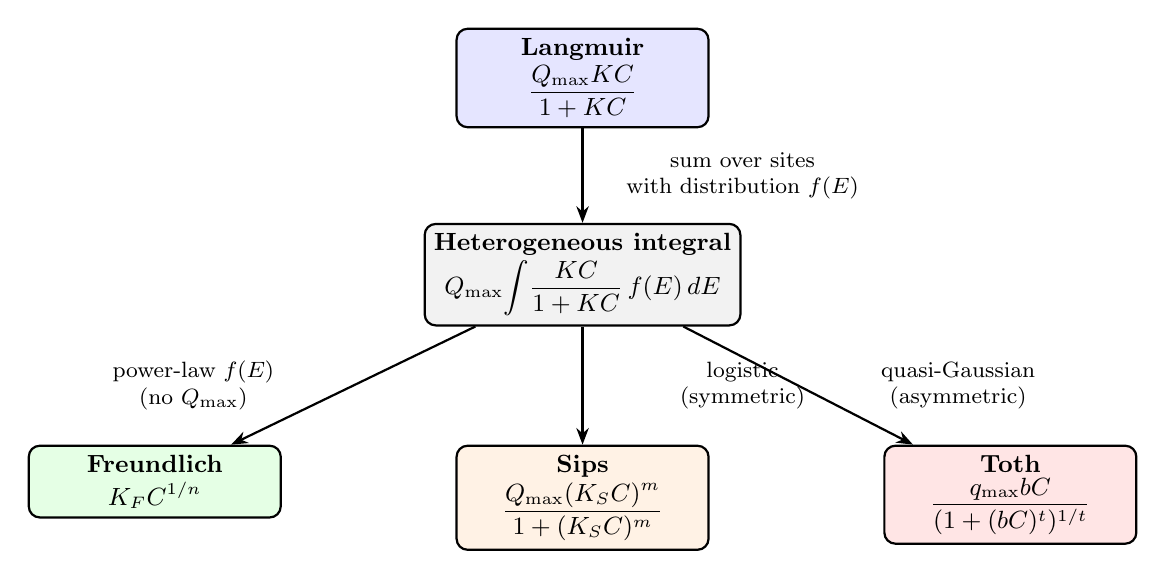
\begin{tikzpicture}[
			every node/.style={font=\small},
			box/.style={draw, rounded corners, minimum width=3.2cm,
				minimum height=0.9cm, align=center, thick},
			arr/.style={-{Stealth[length=6pt]}, thick},
			note/.style={font=\footnotesize, text width=3.8cm, align=center},
			]
			% Root
			\node[box, fill=blue!10] (lang) {\textbf{Langmuir}\\[1pt]$\displaystyle\frac{Q_{\max}KC}{1+KC}$};

			% General heterogeneous
			\node[box, fill=gray!10, below=1.2cm of lang] (het)
			{\textbf{Heterogeneous integral}\\[1pt]$\displaystyle Q_{\max}\!\int\!\frac{KC}{1+KC}\,f(E)\,dE$};

			% Branches
			\node[box, fill=green!10, below left=1.5cm and 1.8cm of het] (freund)
			{\textbf{Freundlich}\\[1pt]$K_F C^{1/n}$};
			\node[box, fill=orange!10, below=1.5cm of het] (sips)
			{\textbf{Sips}\\[1pt]$\displaystyle\frac{Q_{\max}(K_SC)^m}{1+(K_SC)^m}$};
			\node[box, fill=red!10, below right=1.5cm and 1.8cm of het] (toth)
			{\textbf{Toth}\\[1pt]$\displaystyle\frac{q_{\max}bC}{(1+(bC)^t)^{1/t}}$};

			% Arrows
			\draw[arr] (lang) -- (het)
			node[midway, right, note] {sum over sites\\with distribution $f(E)$};
			\draw[arr] (het) -- (freund)
			node[midway, left, note] {power-law $f(E)$\\(no $Q_{\max}$)};
			\draw[arr] (het) -- (sips)
			node[midway, right, note] {logistic\\(symmetric)};
			\draw[arr] (het) -- (toth)
			node[midway, right, note] {quasi-Gaussian\\(asymmetric)};
		\end{tikzpicture}
		\caption{Family of isotherms derived from the local Langmuir model
			by choosing different site-energy distributions~$f(E)$.}
		\label{fig:isotherm_family_tree}
	\end{figure}

	\subsubsection{Derivation of the Freundlich isotherm}

	If the energy distribution follows a power law,
	\begin{equation}
		f(E) = \frac{n}{\pi}\sin(\pi n)\,
		K_0^{\,n}\, \mathrm{e}^{\,nE/RT},
		\qquad 0 < n < 1,
	\end{equation}
	the substitution $y = K(E)\,C_e$ in Eq.~\eqref{eq:general_heterogeneous}
	leads to an integral of the form
	\begin{equation}
		q_e \propto C_e^{\,n}
		\int_{C_e K_0}^{\infty} \frac{y^{-n}}{1 + y}\,\mathrm{d}y.
		\label{eq:freundlich_derivation_step}
	\end{equation}
	In the regime $C_e K_0 \ll 1$, one may extend the lower limit from
	$C_e K_0$ to~$0$ and quantify the incurred error. Indeed,
	\begin{equation}
		\int_{C_e K_0}^{\infty} \frac{y^{-n}}{1+y}\, \mathrm{d}y
		=
		\int_{0}^{\infty} \frac{y^{-n}}{1+y}\, \mathrm{d}y
		-
		\int_{0}^{C_e K_0} \frac{y^{-n}}{1+y}\, \mathrm{d}y,
	\end{equation}
	and the remainder satisfies
	\begin{equation}
		0 \le \int_{0}^{C_e K_0} \frac{y^{-n}}{1+y}\, \mathrm{d}y
		\le \frac{(C_e K_0)^{1-n}}{1-n},
		\qquad 0<n<1,
	\end{equation}
	so the approximation becomes asymptotically exact as $C_e K_0 \to 0$.
	The constant integral is evaluated by the change of variables
	$y = t/(1-t)$, giving
	\begin{align}
		\int_{0}^{\infty} \frac{y^{-n}}{1+y}\, \mathrm{d}y
		&= \int_{0}^{1} t^{(1-n)-1}(1-t)^{n-1}\, \mathrm{d}t
		= B(1-n,\,n) \nonumber\\
		&= \Gamma(1-n)\,\Gamma(n),
		\label{eq:beta_integral_gamma}
	\end{align}
	and Euler's reflection formula $\Gamma(n)\Gamma(1-n) = \pi/\sin(\pi n)$
	yields
	\begin{equation}
		\int_{0}^{\infty} \frac{y^{-n}}{1+y}\, \mathrm{d}y
		= \frac{\pi}{\sin(\pi n)}, \qquad 0<n<1,
		\label{eq:beta_integral}
	\end{equation}
	which leads directly to the Freundlich form
	$q_e = K_F C_e^{1/n}$ (Eq.~\eqref{eq:Freundlich}),
	with $K_F$ absorbing all prefactors. Because the power-law distribution
	is unbounded, no finite $Q_{\max}$ emerges.

	\subsubsection{Derivation of the Sips isotherm}

	If the site-energy distribution is a \emph{logistic} (symmetric)
	density with location~$E_c$ and scale $b = nRT$,
	\begin{equation}
		f(E) = \frac{1}{b}\,
		\frac{\exp\!\bigl(\frac{E - E_c}{b}\bigr)}
		{\Bigl[1 + \exp\!\bigl(\frac{E - E_c}{b}\bigr)\Bigr]^{2}},
		\label{eq:sips_energy_dist}
	\end{equation}
	substitution into Eq.~\eqref{eq:general_heterogeneous} and evaluation
	within the condensation approximation yields
	\begin{equation}
		q_e = \frac{Q_{\max}\,(K_S C_e)^{m}}{1 + (K_S C_e)^{m}},
		\label{eq:Sips_derived}
	\end{equation}
	where $m = 1/n$ is the heterogeneity exponent and
	$K_S = K_0\exp(E_c / RT)$.
	The logistic distribution is symmetric about~$E_c$, so the Sips
	isotherm describes surfaces whose site energies are symmetrically
	distributed around a mean value.
	When $m = 1$ (i.e.\ $n = 1$, zero heterogeneity), the distribution
	collapses to a Dirac delta and Eq.~\eqref{eq:Sips_derived} reduces
	to the single-site Langmuir isotherm.

	\subsubsection{Derivation of the Toth isotherm}

	The Toth isotherm arises when the energy distribution is a
	\emph{quasi-Gaussian, asymmetric} density skewed toward low
	energies. Although no simple closed-form expression for $f(E)$
	exists in this case, the resulting macroscopic isotherm can be
	written as
	\begin{equation}
		q_e = q_{\max}\,
		\frac{b\,C_e}{\bigl[1 + (b\,C_e)^{t}\bigr]^{1/t}},
		\label{eq:Toth_derived}
	\end{equation}
	where $t$ is the heterogeneity parameter ($0 < t \leq 1$) and
	$b$ is an affinity constant. The asymmetry of $f(E)$ distinguishes
	the Toth model from the Sips model: the energy distribution has a
	longer tail toward low adsorption energies, making it more suitable
	for surfaces where the majority of sites are weaker than the mean.
	When $t = 1$, the distribution becomes symmetric and
	Eq.~\eqref{eq:Toth_derived} reduces to the Langmuir isotherm.

	
	
	\section{Freundlich isotherm}
	
	The Freundlich isotherm is an empirical model commonly written as
	\begin{equation}
		q_e = K_F C_e^{1/n},
		\label{eq:Freundlich}
	\end{equation}
	where \(q_e\) is the equilibrium adsorbed amount, \(C_e\) is the
	equilibrium concentration in the fluid phase, \(K_F\) is the
	Freundlich constant related to adsorption capacity, and \(1/n\)
	is a heterogeneity parameter (typically \(0 < 1/n < 1\)).
	
	\subsection{High concentration limit: absence of an intrinsic \(Q_{\max}\)}
	
	In contrast to the Langmuir isotherm, the Freundlich model does not
	contain a built-in saturation capacity. Taking the limit of
	eq.~\eqref{eq:Freundlich} for large \(C_e\),
	\begin{equation}
		\lim_{C_e \to \infty} q_e
		= \lim_{C_e \to \infty} K_F C_e^{1/n}.
	\end{equation}
	For any fixed \(K_F > 0\) and \(1/n > 0\), we have
	\begin{equation}
		\lim_{C_e \to \infty} C_e^{1/n} = \infty,
	\end{equation}
	so that
	\begin{equation}
		\lim_{C_e \to \infty} q_e = \infty.
	\end{equation}
	Therefore, the Freundlich isotherm does not predict a finite
	saturation capacity:
	\begin{equation}
		\boxed{
			\text{Freundlich has no intrinsic } Q_{\max};
			\quad
			\lim_{C_e \to \infty} q_e = \infty.
		}
	\end{equation}
	
	In practical applications, one sometimes introduces an
	\emph{effective} or \emph{operational} saturation capacity by
	restricting the validity of the Freundlich model to a maximum
	concentration \(C_{\max}\) (for example, the upper limit of the
	experimental range). In that case, an effective capacity may be
	defined as
	\begin{equation}
		Q_{\max}^{\mathrm{(F,eff)}} = q_e(C_{\max})
		= K_F C_{\max}^{1/n},
	\end{equation}
	which should be understood as a phenomenological quantity, not
	a true thermodynamic saturation.
	
	\subsection{Low concentration behavior: comparison with Henry law}
	
	Henry law for dilute solutions is written as
	\begin{equation}
		q_e \approx K_H C_e,
		\label{eq:Henry}
	\end{equation}
	with \(K_H\) the Henry constant, equal to the initial slope of the
	isotherm at \(C_e \to 0\):
	\begin{equation}
		K_H = \left. \frac{\mathrm{d} q_e}{\mathrm{d} C_e}\right|_{C_e \to 0}.
	\end{equation}
	
	For the Freundlich isotherm, the derivative of \(q_e\) is
	\begin{equation}
		\frac{\mathrm{d} q_e}{\mathrm{d} C_e}
		= K_F \frac{1}{n} C_e^{1/n - 1}.
	\end{equation}
	Taking the limit as \(C_e \to 0\),
	\begin{equation}
		\lim_{C_e \to 0}
		\frac{\mathrm{d} q_e}{\mathrm{d} C_e}
		= \lim_{C_e \to 0}
		K_F \frac{1}{n} C_e^{1/n - 1}.
	\end{equation}
	The behavior depends critically on the exponent \(1/n\):
	
	\begin{itemize}
		\item If \(1/n = 1\), then \(q_e = K_F C_e\) and
		\begin{equation}
			\frac{\mathrm{d} q_e}{\mathrm{d} C_e} = K_F,
		\end{equation}
		so that
		\begin{equation}
			K_H = K_F,
		\end{equation}
		and the Freundlich isotherm reduces exactly to Henry law.
		
		\item If \(1/n < 1\), which is the usual case in heterogeneous
		systems, then \(1/n - 1 < 0\) and
		\begin{equation}
			\lim_{C_e \to 0} C_e^{1/n - 1} = \infty,
		\end{equation}
		so that
		\begin{equation}
			\lim_{C_e \to 0}
			\frac{\mathrm{d} q_e}{\mathrm{d} C_e} = \infty.
		\end{equation}
		In this regime, the isotherm is more than linear at low concentration,
		and a finite Henry constant in the strict sense does not exist.
		
		\item If \(1/n > 1\), then \(1/n - 1 > 0\) and
		\begin{equation}
			\lim_{C_e \to 0} C_e^{1/n - 1} = 0,
		\end{equation}
		so that
		\begin{equation}
			\lim_{C_e \to 0}
			\frac{\mathrm{d} q_e}{\mathrm{d} C_e} = 0.
		\end{equation}
		The isotherm is sublinear at low concentration and again does not
		have a constant nonzero Henry slope.
	\end{itemize}
	
	Thus, in general, the Freundlich model does not admit a unique,
	concentration-independent Henry constant, except in the special
	case \(1/n = 1\). Instead, one can define a \emph{local} or
	\emph{apparent} Henry coefficient as
	\begin{equation}
		K_H(C_e) = \frac{q_e}{C_e}
		= \frac{K_F C_e^{1/n}}{C_e}
		= K_F C_e^{1/n - 1},
	\end{equation}
	which explicitly depends on concentration and diverges or vanishes
	as \(C_e \to 0\) depending on the value of \(1/n\).
	
	\subsection{Affinity constant and adsorption free energy}
	
	For thermodynamic interpretation, it is convenient to identify an
	\emph{affinity constant} at a chosen reference concentration
	\(C^{\dagger}\) within the experimentally relevant range. A
	natural choice is the local Henry coefficient at \(C^{\dagger}\),
	\begin{equation}
		K_{\mathrm{aff}}\!\left(C^{\dagger}\right)
		= K_H\!\left(C^{\dagger}\right)
		= K_F \left(C^{\dagger}\right)^{1/n - 1}.
	\end{equation}
	This quantity has the same role as the Langmuir constant in the
	dilute limit, but it is explicitly associated with a given
	concentration \(C^{\dagger}\) and reflects the heterogeneity
	encoded in the exponent \(1/n\).
	
	To convert \(K_{\mathrm{aff}}\) into a dimensionless equilibrium
	constant, we introduce a standard concentration \(C^0\) (for example
	\(1~\mathrm{mol~L^{-1}}\)) and define
	\begin{equation}
		K_{\mathrm{aff}}^{\ast}\!\left(C^{\dagger}\right)
		= K_{\mathrm{aff}}\!\left(C^{\dagger}\right) C^0
		= K_F C^0 \left(C^{\dagger}\right)^{1/n - 1}.
	\end{equation}
	The associated standard Gibbs free energy of adsorption, evaluated
	at the reference concentration \(C^{\dagger}\), is then
	\begin{equation}
		\Delta G_{\mathrm{ads}}^{0}\!\left(C^{\dagger}\right)
		= - R T
		\ln K_{\mathrm{aff}}^{\ast}\!\left(C^{\dagger}\right)
		= - R T
		\ln\!\left[
		K_F C^0 \left(C^{\dagger}\right)^{1/n - 1}
		\right].
	\end{equation}
	An adsorption affinity energy may be defined as the magnitude of
	this free energy:
	\begin{equation}
		E_{\mathrm{aff}}\!\left(C^{\dagger}\right)
		= - \Delta G_{\mathrm{ads}}^{0}\!\left(C^{\dagger}\right)
		= R T
		\ln\!\left[
		K_F C^0 \left(C^{\dagger}\right)^{1/n - 1}
		\right].
	\end{equation}
	
	Therefore, while the Langmuir isotherm provides a single,
	concentration-independent affinity constant and a well-defined
	saturation capacity \(Q_{\max}\), the Freundlich isotherm describes
	a heterogeneous adsorption system in which:
	
	\begin{itemize}
		\item There is no intrinsic \(Q_{\max}\); only an effective
		\(Q_{\max}^{\mathrm{(F,eff)}}\) can be defined by restricting the
		concentration range.
		
		\item The low-concentration behavior does not, in general, reduce
		to a simple Henry law with a constant \(K_H\); instead, one obtains
		a concentration-dependent local Henry coefficient
		\(K_H(C_e) = K_F C_e^{1/n - 1}\).
		
		\item The adsorption free energy and affinity energy are naturally
		defined as concentration-dependent quantities,
		\(\Delta G_{\mathrm{ads}}^{0}(C^{\dagger})\) and
		\(E_{\mathrm{aff}}(C^{\dagger})\), evaluated at a chosen reference
		concentration \(C^{\dagger}\), reflecting the distribution of
		adsorption energies inherent to the Freundlich model.
	\end{itemize}
	
	\subsection{Apparent adsorption free energy}
	
	Following the Langmuir case, one can define an apparent standard free energy
	of adsorption at a chosen reference concentration $C_{\mathrm{ref}}$ by using
	$K_H^{\mathrm{app}}(C_{\mathrm{ref}})$ as an effective equilibrium constant.
	Introducing a standard concentration $C^0$ (typically
	$1~\mathrm{mol\,L^{-1}}$), the dimensionless effective constant is
	\begin{equation}
		K_{\mathrm{eff}}^{\ast}
		= K_H^{\mathrm{app}}(C_{\mathrm{ref}})\, C^0,
	\end{equation}
	and the corresponding apparent standard Gibbs free energy is
	\begin{equation}
		\Delta G_{\mathrm{ads}}^{0,\mathrm{app}}(C_{\mathrm{ref}})
		= - R T \ln K_{\mathrm{eff}}^{\ast}
		= - R T \ln\!\left[ \frac{1}{n} K_F C_{\mathrm{ref}}^{1/n - 1} C^0 \right].
	\end{equation}
	This expression shows explicitly that the adsorption free energy associated
	with a Freundlich isotherm is not unique, but depends on the chosen reference
	concentration $C_{\mathrm{ref}}$. This is a direct consequence of the
	heterogeneous, non-Langmuir nature of the Freundlich model.
	
	In summary, while a single, well-defined adsorption free energy can be
	associated with a Langmuir isotherm, a Freundlich isotherm corresponds
	instead to a distribution of adsorption energies, and only concentration-dependent
	apparent free energies can be defined.
	
	\section{Alternatives to Freundlich model}
	
	\subsection{Sips (Langmuir--Freundlich) isotherm }
	
	A common way to introduce a finite saturation capacity while retaining
	the heterogeneous character of the Freundlich isotherm is the
	Sips (or Langmuir--Freundlich) model:
	\begin{equation}
		q_e = \frac{Q_{\max} K_S C_e^{m}}{1 + K_S C_e^{m}},
		\label{eq:Sips}
	\end{equation}
	where \(Q_{\max}\) is the saturation capacity, \(K_S\) is an affinity
	constant, and \(m\) is a heterogeneity parameter
	(\(0 < m \leq 1\)).
	
	\subsection{High concentration limit: finite \(Q_{\max}\)}
	
	Taking the limit \(C_e \to \infty\) in eq.~\eqref{eq:Sips}:
	\begin{equation}
		\lim_{C_e \to \infty} q_e
		= \lim_{C_e \to \infty}
		\frac{Q_{\max} K_S C_e^{m}}{1 + K_S C_e^{m}}
		= Q_{\max}.
	\end{equation}
	Therefore, the Sips isotherm retains a well defined saturation capacity:
	\begin{equation}
		\boxed{
			\displaystyle \lim_{C_e \to \infty} q_e = Q_{\max}.
		}
	\end{equation}
	
	\subsection{Low concentration limit: Freundlich--type behavior}
	
	For small \(C_e\), such that \(K_S C_e^{m} \ll 1\), we can expand
	the denominator in eq.~\eqref{eq:Sips}:
	\begin{equation}
		\frac{1}{1 + K_S C_e^{m}}
		\approx 1 - K_S C_e^{m} + \mathcal{O}(C_e^{2m}).
	\end{equation}
	Keeping only the first order in \(C_e^{m}\),
	\begin{equation}
		q_e \approx Q_{\max} K_S C_e^{m}.
	\end{equation}
	This has the Freundlich form
	\begin{equation}
		q_e \approx K_F C_e^{1/n},
	\end{equation}
	if we identify
	\begin{equation}
		K_F = Q_{\max} K_S, \qquad \frac{1}{n} = m.
	\end{equation}
	Thus, at low concentrations the Sips isotherm behaves as a
	Freundlich model with parameters \(K_F\) and \(1/n = m\), while at
	high concentrations it saturates at \(Q_{\max}\) like a Langmuir
	isotherm. In this sense, Sips interpolates between Freundlich and
	Langmuir.
	
	\subsection{Comparison of the initial slope and Henry constant}
	
	As in the traditional Freundlich model with \(1/n \neq 1\), the
	initial slope at \(C_e \to 0\) is not finite if \(m \neq 1\). The
	ratio \(q_e / C_e\) at low concentration is
	\begin{equation}
		\frac{q_e}{C_e}
		\approx Q_{\max} K_S C_e^{m-1}.
	\end{equation}
	Therefore, an apparent local Henry coefficient can be defined as
	\begin{equation}
		K_H(C_e)
		= \frac{q_e}{C_e}
		= Q_{\max} K_S C_e^{m - 1},
	\end{equation}
	which reduces to a constant only for the Langmuir limit \(m = 1\).
	For \(m \neq 1\) this local Henry coefficient is concentration
	dependent, as in the Freundlich case, but now embedded in a model
	with finite \(Q_{\max}\).
	
	\subsubsection{Energy distribution}
	
	For practical comparison of affinity constants, a formal ``affinity energy'' can be defined from an effective equilibrium constant of adsorption as
	\begin{equation}
		\Delta G_{\mathrm{ads}} \;=\; -\,RT\,\ln\!\big(K_{\mathrm{eq}}\,C^\circ\big),
	\end{equation}
	where \(C^\circ\) is a reference concentration chosen within the experimental range (for example, \(1~\mathrm{ppm}\)) so that the argument of the logarithm is dimensionless. The corresponding positive affinity energy is
	\begin{equation}
		E_0 \;\equiv\; -\,\Delta G_{\mathrm{ads}}
		\quad\Rightarrow\quad
		\frac{E_0}{RT} \;=\; \ln\!\big(K_{\mathrm{eq}}\,C^\circ\big).
		\label{eq:E_def}
	\end{equation}
	Although \(K_{\mathrm{eq}}\) in adsorption models is typically an empirical parameter rather than a strict thermodynamic equilibrium constant, Eq.~\eqref{eq:E_def} provides a consistent framework to compare materials on a relative energetic scale.
	
	Applying Eq.~\eqref{eq:E_def} to the Langmuir and Sips isotherms defined in Eqs.~\eqref{eq:langmuir_nonlin} and \eqref{eq:SIPS_nonlin}, respectively:
	
	\paragraph{Langmuir isotherm.}
	
	For the Langmuir isotherm,
	\begin{equation}
		q_e \;=\; \frac{Q_{\max}\,K_L\,C_e}{1 + K_L\,C_e},
	\end{equation}
	the Langmuir constant \(K_L\) has units \([C]^{-1}\), so that \(K_L C^\circ\) is dimensionless and can be directly used in Eq.~\eqref{eq:E_def}:
	\begin{equation}
		\text{Langmuir:}\qquad
		\frac{E_0}{RT} \;=\; \ln\!\big(K_L\,C^\circ\big).
		\label{eq:E_langmuir}
	\end{equation}
	
	\paragraph{Sips (Langmuir--Freundlich) isotherm.}
	
	For the Sips isotherm in the form
	\begin{equation}
		q_e \;=\; \frac{Q_{\max}\,K_S\,C_e^{n}}{1 + K_S\,C_e^{n}},
	\end{equation}
	the Sips constant \(K_S\) has units \([C]^{-n}\), such that the product \(K_S C_e^{n}\) is dimensionless. To compare Sips and Langmuir on the same energetic basis, it is convenient to define an effective equilibrium constant with units \([C]^{-1}\):
	\begin{equation}
		K_{\mathrm{eq}}^{\mathrm{(Sips)}} \;=\; K_S^{1/n}.
	\end{equation}
	Inserting \(K_{\mathrm{eq}}^{\mathrm{(Sips)}}\) into Eq.~\eqref{eq:E_def} gives
	\begin{align}
		\frac{E_0}{RT}
		\;&=\; \ln\!\big(K_{\mathrm{eq}}^{\mathrm{(Sips)}}\,C^\circ\big)
		\;=\; \ln\!\big(K_S^{1/n}\,C^\circ\big) \nonumber\\[4pt]
		\;&=\; \frac{1}{n}\,\ln K_S \;+\; \ln C^\circ
		\;=\; \frac{1}{n}\,\ln\!\big(K_S\,(C^\circ)^{n}\big).
		\label{eq:E_sips}
	\end{align}
	Thus, for the Sips isotherm,
	\begin{equation}
		\text{Sips:}\qquad
		\frac{E_0}{RT} \;=\; \frac{1}{n}\,\ln\!\big(K_S\,(C^\circ)^{n}\big),
	\end{equation}
	where the factor \(1/n\) explicitly appears outside the logarithm to preserve correct units and to account for the empirical heterogeneity exponent. In the limit \(n = 1\), \(K_S\) reduces to \(K_L\) and Eq.~\eqref{eq:E_sips} collapses to the Langmuir expression in Eq.~\eqref{eq:E_langmuir}.
	
	In both cases, larger values of \(E_0/RT\) correspond to stronger adsorption affinity and therefore indicate a more favorable adsorption process. For the Sips model, this affinity should be interpreted as an effective quantity that incorporates the distribution of adsorption energies encoded in the exponent \(n\).
	
	\subsubsection{Energy distribution for the Sips isotherm in concentration form}
	
	We consider the Sips isotherm written in terms of equilibrium concentration
	\(C_e\) as
	\begin{equation}
		q(C_e)
		\;=\;
		\frac{Q_{\max}\,\bigl(K_S C_e\bigr)^{1/n}}
		{1 + \bigl(K_S C_e\bigr)^{1/n}},
		\label{eq:Sips_C}
	\end{equation}
	where \(Q_{\max}\) is the saturation capacity, \(K_S\) is the Sips affinity
	constant (with units \([C]^{-1}\)), and \(1/n\) is the empirical
	heterogeneity exponent.
	
	To connect this isotherm with an adsorption energy distribution in the
	condensation approximation, we introduce an effective relation between
	concentration and adsorption energy,
	\begin{equation}
		C_e
		\;=\;
		C^{\ast}\,\exp\!\left(-\frac{E}{RT}\right),
		\label{eq:cond_approx_C}
	\end{equation}
	where \(C^{\ast}\) is a reference concentration (for example, a
	characteristic or saturation concentration in the liquid phase), \(E\) is
	an adsorption energy, and \(R\) and \(T\) are the gas constant and absolute
	temperature, respectively. The ratio \(C_e/C^{\ast}\) is then
	dimensionless, as required.
	
	Substituting eq.~\eqref{eq:cond_approx_C} into eq.~\eqref{eq:Sips_C},
	\begin{align}
		q(E)
		\;&=\;
		\frac{Q_{\max}\,\bigl[K_S C^{\ast}\exp(-E/RT)\bigr]^{1/n}}
		{1 + \bigl[K_S C^{\ast}\exp(-E/RT)\bigr]^{1/n}}
		\nonumber\\[4pt]
		\;&=\;
		\frac{Q_{\max}\,A^{1/n}\,\exp\bigl(-E/(nRT)\bigr)}
		{1 + A^{1/n}\,\exp\bigl(-E/(nRT)\bigr)},
	\end{align}
	where we have defined
	\begin{equation}
		A = K_S C^{\ast}.
	\end{equation}
	Let
	\begin{equation}
		B = A^{1/n} = \bigl(K_S C^{\ast}\bigr)^{1/n}.
	\end{equation}
	Then
	\begin{equation}
		q(E)
		\;=\;
		\frac{Q_{\max}\,B\,\exp\bigl(-E/(nRT)\bigr)}
		{1 + B\,\exp\bigl(-E/(nRT)\bigr)}.
	\end{equation}
	Multiplying numerator and denominator by \(\exp\bigl(E/(nRT)\bigr)\),
	\begin{equation}
		q(E)
		\;=\;
		\frac{Q_{\max}\,B}
		{\exp\bigl(E/(nRT)\bigr) + B}.
	\end{equation}
	It is convenient to define a characteristic energy \(E_c\) such that
	\begin{equation}
		E_c = nRT\,\ln B
		= nRT\,\ln\bigl(K_S C^{\ast}\bigr)^{1/n}
		= RT\,\ln\bigl(K_S C^{\ast}\bigr),
	\end{equation}
	so that
	\begin{equation}
		\exp\!\left(\frac{E}{nRT}\right) + B
		\;=\;
		B\left[1 + \exp\!\left(\frac{E - E_c}{nRT}\right)\right].
	\end{equation}
	Then
	\begin{equation}
		q(E)
		\;=\;
		\frac{Q_{\max}}
		{1 + \exp\!\left(\dfrac{E - E_c}{nRT}\right)}.
		\label{eq:qE_logistic_conc}
	\end{equation}
	Thus, the coverage as a function of energy is a logistic cumulative
	distribution function (CDF) centered at \(E_c\), with scale parameter
	\(b = nRT\). Notice that \(E_c\) is the energy at which \(q(E_c) = Q_{\max}/2\).
	
	Within the condensation approximation, the site energy distribution
	\(f(E)\) is obtained from
	\begin{equation}
		f(E) = -\,\frac{\mathrm{d}q(E)}{\mathrm{d}E}.
	\end{equation}
	Differentiating eq.~\eqref{eq:qE_logistic_conc},
	\begin{equation}
		f(E)
		\;=\;
		\frac{Q_{\max}}{nRT}\,
		\frac{\exp\!\left(\dfrac{E - E_c}{nRT}\right)}
		{\left[1 + \exp\!\left(\dfrac{E - E_c}{nRT}\right)\right]^{2}}.
		\label{eq:fE_logistic_conc}
	\end{equation}
	Defining the dimensionless variable
	\begin{equation}
		u = \frac{E - E_c}{b},
		\qquad
		b = nRT,
	\end{equation}
	eq.~\eqref{eq:fE_logistic_conc} can be written as
	\begin{equation}
		f(E)
		\;=\;
		Q_{\max}\,\frac{1}{b}\,g(u),
		\qquad
		g(u) = \frac{\exp(u)}{\bigl[1 + \exp(u)\bigr]^{2}}.
	\end{equation}
	The normalized energy distribution
	\(\phi(E) = f(E)/Q_{\max}\) is therefore a logistic probability density
	with location \(E_c\) and scale \(b = nRT\).
	
	The variance of a logistic distribution with scale \(b\) is
	\(\sigma_E^{2} = \pi^{2} b^{2} / 3\). Hence, in terms of the Sips
	heterogeneity parameter \(1/n\),
	\begin{equation}
		\sigma_E
		\;=\;
		\frac{\pi}{\sqrt{3}}\,b
		\;=\;
		\frac{\pi}{\sqrt{3}}\,nRT.
		\label{eq:sigmaE_n_conc}
	\end{equation}
	Thus, the Sips exponent \(1/n\) directly controls the width of the
	adsorption energy distribution: larger \(n\) (smaller \(1/n\)) leads
	to a broader distribution of energies, while smaller \(n\) (larger
	\(1/n\)) corresponds to a narrower distribution.
	
	Since the logistic distribution is very similar in shape to a normal
	distribution, the Sips energy distribution can be approximated as
	\begin{equation}
		\phi(E)
		\;\approx\;
		\frac{1}{\sqrt{2\pi}\,\sigma_E}
		\exp\!\left[
		-\,\frac{\bigl(E - E_c\bigr)^{2}}{2\sigma_E^{2}}
		\right],
	\end{equation}
	with mean energy \(E_c = RT \ln(K_S C^{\ast})\) and standard deviation
	\(\sigma_E = (\pi/\sqrt{3})\,nRT\). In this representation, the Sips
	heterogeneity parameter \(1/n\) is directly mapped onto the dispersion
	of adsorption energies in concentration space.
	
	
	\subsection{Toth isotherm}
	\[
	q_e = q_{\max} \frac{b C_e}{\left(1 + (b C_e)^{t}\right)^{1/t}}
	\]
	
	\subsubsection{High concentration limit: finite $Q_{\max}$}
	
	For $b C_e \gg 1$, the Toth isotherm
	\[
	q_e = q_{\max} \frac{b C_e}{\left(1 + (b C_e)^{t}\right)^{1/t}}
	\]
	reduces to
	\begin{align}
		q_e 
		&= q_{\max} \frac{b C_e}{\left[1 + (b C_e)^{t}\right]^{1/t}}
		\simeq q_{\max} \frac{b C_e}{\left[(b C_e)^{t}\right]^{1/t}} \nonumber \\
		&= q_{\max} \frac{b C_e}{b C_e}
		= q_{\max}.
	\end{align}
	Thus, at high equilibrium concentration, the Toth model predicts a finite saturation capacity, $Q_{\max} = q_{\max}$.
	
	\subsubsection{Low concentration limit}
	
	For $b C_e \ll 1$, the Toth isotherm
	\[
	q_e = q_{\max} \frac{b C_e}{\left(1 + (b C_e)^{t}\right)^{1/t}}
	\]
	can be expanded using
	\[
	\left(1 + x\right)^{-1/t} \simeq 1 - \frac{x}{t} \quad \text{for } |x| \ll 1,
	\]
	with $x = (b C_e)^{t}$. Thus,
	\begin{align}
		q_e
		&= q_{\max} b C_e \left(1 + (b C_e)^{t}\right)^{-1/t} \nonumber \\
		&\simeq q_{\max} b C_e \left[1 - \frac{(b C_e)^{t}}{t}\right].
	\end{align}
	To first order in $C_e$, one obtains
	\begin{equation}
		q_e \simeq q_{\max} b\, C_e,
	\end{equation}
	that is, a Henry-type behavior with an effective Henry constant
	\begin{equation}
		K_H^{\mathrm{eff}} = q_{\max} b.
	\end{equation}
	
	
	% \subsection{Keller-Staudt-Toth (KST) isotherm}
	% \[
	% q_e = q_{\max} \frac{b C_e}{\left[1 + (b C_e)^{a}\right]^{1/a}}
	%  \]
	
	\subsection{Jovanovich isotherm}
	\[
	q_e = q_{\max} \left[1 - \exp(-b C_e)\right]
	\]
	
	\subsubsection{High concentration limit: finite $Q_{\max}$}
	
	For $b C_e \gg 1$, the exponential term vanishes,
	\[
	\exp(-b C_e) \to 0,
	\]
	and the Jovanovich isotherm
	\[
	q_e = q_{\max} \left[1 - \exp(-b C_e)\right]
	\]
	reduces to
	\begin{align}
		q_e 
		&= q_{\max} \left[1 - \exp(-b C_e)\right] \nonumber \\
		&\simeq q_{\max} (1 - 0) \nonumber \\
		&= q_{\max}.
	\end{align}
	Thus, at high equilibrium concentration, the Jovanovich model predicts a finite saturation capacity, $Q_{\max} = q_{\max}$.
	
	\subsubsection{Low concentration limit}
	
	For $b C_e \ll 1$, the exponential can be expanded as
	\[
	\exp(-b C_e) \simeq 1 - b C_e + \frac{(b C_e)^2}{2} + \cdots.
	\]
	Substituting into the Jovanovich isotherm,
	\begin{align}
		q_e
		&= q_{\max} \left[1 - \exp(-b C_e)\right] \nonumber \\
		&\simeq q_{\max} \left[1 - \left(1 - b C_e + \frac{(b C_e)^2}{2}\right)\right] \nonumber \\
		&= q_{\max} \left[b C_e - \frac{(b C_e)^2}{2}\right].
	\end{align}
	To first order in $C_e$, one obtains
	\begin{equation}
		q_e \simeq q_{\max} b\, C_e,
	\end{equation}
	that is, a Henry-type behavior with an effective Henry constant
	\begin{equation}
		K_H^{\mathrm{eff}} = q_{\max} b.
	\end{equation}
	
	
	\subsection{Temkin isotherm}
	\[
	q_e = \frac{RT}{b_T} \ln(a_T C_e)
	\]
	
	\subsubsection{Nature of the model}
	
	The Temkin isotherm is usually regarded as a semi-empirical model. It can be
	derived by assuming that the adsorption energy decreases linearly with surface
	coverage, but in practice it is mainly used as an empirical two-parameter
	correlation valid over an intermediate range of $C_e$.
	
	\subsubsection{High concentration limit: no finite $Q_{\max}$}
	
	For $C_e \to \infty$,
	\begin{align}
		q_e 
		&= \frac{RT}{b_T} \ln(a_T C_e) \nonumber \\
		&= \frac{RT}{b_T} \left[\ln a_T + \ln C_e\right]
		\;\xrightarrow[C_e \to \infty]{}\; +\infty.
	\end{align}
	Thus, the Temkin model does not predict a finite saturation capacity, that is, there is no finite $Q_{\max}$ in this limit.
	
	Therefore, the Temkin isotherm is best viewed as an approximate description of adsorption over a limited, intermediate concentration range.
	
	\subsubsection{Low concentration limit}
	
	For $C_e \to 0$, one has
	\[
	\ln(a_T C_e) = \ln a_T + \ln C_e \xrightarrow[C_e \to 0]{} -\infty,
	\]
	and therefore
	\[
	q_e = \frac{RT}{b_T} \ln(a_T C_e) \xrightarrow[C_e \to 0]{} -\infty,
	\]
	which is not physically meaningful for adsorption. The Temkin isotherm is thus intended to describe an intermediate coverage range, not the strict $C_e \to 0$ or $C_e \to \infty$ limits.
	
	A local, effective Henry constant around a reference concentration $C_{e,\mathrm{ref}}$ can be obtained from the slope
	\[
	K_H^{\mathrm{eff}}(C_{e,\mathrm{ref}})
	= \left.\frac{d q_e}{d C_e}\right|_{C_e = C_{e,\mathrm{ref}}}
	= \frac{RT}{b_T C_{e,\mathrm{ref}}}.
	\].
	
	
	\subsection{Unilan isotherm}
	\[
	q_e = q_{\max} \int_{-s}^{s} \frac{b_0 \exp(-\alpha E)\, C_e}{1 + b_0 \exp(-\alpha E)\, C_e} \, dE
	\]
	
	\subsubsection{Nature of the model}
	
	The Unilan (uniform-energy Langmuir) isotherm describes adsorption on a
	heterogeneous surface by superposing local Langmuir contributions over a
	continuous distribution of adsorption energies $E$. The factor
	$\exp(-\alpha E)$ weights the local affinity $b_0$ according to the energy,
	and the integral represents the contribution of all site types. In this way,
	$q_{\max}$ is the overall saturation capacity, while $b_0$, $\alpha$, and $s$
	encode the shape and width of the energy distribution.
	
	\subsubsection{High concentration limit: finite $Q_{\max}$}
	
	For $b_0 \exp(-\alpha E)\, C_e \gg 1$ over the whole energy range,
	\[
	\frac{b_0 \exp(-\alpha E)\, C_e}{1 + b_0 \exp(-\alpha E)\, C_e} \to 1,
	\]
	and the Unilan isotherm reduces to
	\begin{equation}
		q_e \simeq q_{\max} \int_{-s}^{s} 1 \, dE.
	\end{equation}
	If the energy distribution is normalized so that
	\[
	\int_{-s}^{s} dE = 1,
	\]
	then
	\begin{equation}
		q_e \to q_{\max} \equiv Q_{\max},
	\end{equation}
	and the model predicts a finite saturation capacity.
	
	\subsubsection{Low concentration limit}
	
	For $b_0 \exp(-\alpha E)\, C_e \ll 1$, the local Langmuir term can be
	linearized as
	\[
	\frac{b_0 \exp(-\alpha E)\, C_e}{1 + b_0 \exp(-\alpha E)\, C_e}
	\simeq b_0 \exp(-\alpha E)\, C_e.
	\]
	Then
	\begin{align}
		q_e
		&\simeq q_{\max} \int_{-s}^{s} b_0 \exp(-\alpha E)\, C_e \, dE \nonumber \\
		&= q_{\max} b_0 C_e \int_{-s}^{s} \exp(-\alpha E)\, dE.
	\end{align}
	To first order in $C_e$, one obtains a Henry-type behavior
	\begin{equation}
		q_e \simeq K_H^{\mathrm{eff}}\, C_e,
	\end{equation}
	with an effective Henry constant
	\begin{equation}
		K_H^{\mathrm{eff}} = q_{\max} b_0 \int_{-s}^{s} \exp(-\alpha E)\, dE.
	\end{equation}
	
	
	\subsection{Distribution broadening in function of temperature}
	
	\subsection{Error handling}
	
	
	\subsection{Statistical comparison}
	\subsubsection{Two models}
	\subsubsection{Several models}
	\subsubsection{Clustering}
	\paragraph{KNN}
	\paragraph{SVM}
	
	\subsection{Isotherm construction recommendations}
	\subsubsection{Examples}
	\subsection{Plot of variables}
	
	\begin{itemize}
		\item Number of points
	\end{itemize}
	
\end{document}
